\documentclass[a4paper, 12pt, titlepage]{report}
\usepackage{amsmath, amssymb}
\usepackage{graphicx}
\usepackage{caption}
\usepackage{appendix}
\usepackage{chngcntr}
\usepackage{hyperref}
\usepackage{multirow}
\usepackage[left=20mm,right=20mm,top=15mm,bottom=15mm]{geometry}
\usepackage[backend=biber]{biblatex}
\addbibresource{bibli.bib}

\counterwithout{figure}{chapter}
\counterwithout{table}{chapter}
\counterwithout{equation}{chapter}

\begin{document}
\title{EE466: Power Electronics, Machines and Applications Coursework 2}
\author{Scott McBride}
\date{\today}
\maketitle
\tableofcontents
\chapter{Introduction}
This coursework submission shows the worked solutions for part 2 of the coursework assessment. Each question within this corresponds to the relevant question from the coursework specification. Where necessary, additional context is provided to clarify any assumptions within the design processes along with any relevant information provided within the brief.

All relevant files for this submission are contained within the GitHub Repository at this \href{https://github.com/WithASideOfSalt/EE466-Coursework-2}{link}.

\chapter{Question 1}
\section{Context}
This question looks at the Thermal energy transfer between 2 heat sources contained within the same system. Contained within Table~\ref{tab:question1} are the relevant parameters for the system, those being the IGBT, Diode, heatsink and ambient temperature provided by~\cite{EE466CourseworkPart2}

\begin{table}[htbp]
    \centering
    \caption{Parameters for Question 1}
    \label{tab:question1}
    \begin{tabular}{|c|c|c|}
        \hline
        \textbf{Component} & \textbf{Parameter} & \textbf{Value} \\
        \hline
        \multirow{3}{*}{IGBT}
        & Power Dissipation \(W_{\mathrm{IGBT}}\) & 12 W \\
        & Junction-to-case thermal resistance \(R_{\theta jc}\) & \(0.6\,^\circ\mathrm{C/W}\) \\
        & Case-to-heatsink thermal resistance \(R_{\theta chs}\) & \(1.4\,^\circ\mathrm{C/W}\) \\
        \hline
        \multirow{3}{*}{Diode}
        & Power Dissipation \(W_{\mathrm{Diode}}\) & 7 W \\
        & Junction-to-case thermal resistance \(R_{\theta jc}\) & \(0.9\,^\circ\mathrm{C/W}\) \\
        & Case-to-heatsink thermal resistance \(R_{\theta chs}\) & \(1.5\,^\circ\mathrm{C/W}\) \\
        \hline
        \multirow{3}{*}{Heatsink}
        & Heatsink-to-ambient thermal resistance \(R_{\theta hsa}\) & \(3.2\,^\circ\mathrm{C/W}\) \\
        & Thermal capacitance \(C_{\theta hs}\) & \(280\,\mathrm{J/}{}^\circ\mathrm{C}\) \\
        & Ambient temperature & \(40\,^\circ\mathrm{C}\) \\
        \hline
    \end{tabular}
\end{table}

\section{1a}
i) For this question a thermal circuit was to be sketched to represent the system. The thermal circuit is shown in Figure~\ref{fig:question1a}.
\begin{figure}[h]
    \centering
    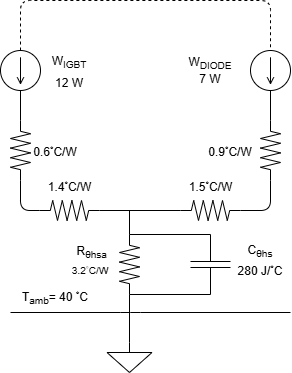
\includegraphics[width=0.4\textwidth]{./Images/Q1Ai.png}
    \caption{Thermal Equivalent Circuit for Question 1ai}
    \label{fig:question1a}
\end{figure}
\\
This thermal circuit shows the IGBT and Diode as two separate heat sources with differing paths to ambient. The relevant thermal resistances are shown along with the thermal capacitance of the heatsink. The ambient temperature is also shown as a reference point for the system.
\vspace{0.5cm}

ii) For this question, the steady state temperature for both the diode and IGBT junctions were to be calculated. To begin the temperature for the heatsink was calculated shown in Equation~\ref{eq:heatsink_temp}.
\begin{equation}
    \begin{split}
            T_{\mathrm{hs}} &= T_{\mathrm{ambient}} + (W_{\mathrm{IGBT}} + W_{\mathrm{Diode}}) \cdot R_{\theta hsa} \\
        &= 40 + (12 + 7) \cdot 3.2 = 100.8\,^\circ\mathrm{C}
    \label{eq:heatsink_temp}
    \end{split}
\end{equation}

With the general temperature of the heatsink calculated, the junction temperatures for both the IGBT and Diode can be calculated using the relevant thermal resistances. The junction temperature for the IGBT is shown in Equation~\ref{eq:igbt_temp}.
\begin{equation}
    \begin{split}
        T_{\mathrm{IGBT}} &= T_{\mathrm{hs}} + W_{\mathrm{IGBT}} \cdot (R_{\theta jc} + R_{\theta chs}) \\
        &= 100.8 + 12 \cdot (0.6 + 1.4) = 124.8\,^\circ\mathrm{C}
    \label{eq:igbt_temp}
    \end{split}
\end{equation}   

The junction temperature for the Diode is shown in Equation~\ref{eq:diode_temp}.
\begin{equation}
    \begin{split}
        T_{\mathrm{Diode}} &= T_{\mathrm{hs}} + W_{\mathrm{Diode}} \cdot (R_{\theta jc} + R_{\theta chs}) \\
        &= 100.8 + 7 \cdot (0.9 + 1.5) = 118.8\,^\circ\mathrm{C}
    \label{eq:diode_temp}
    \end{split}
\end{equation}

\vspace{0.5cm}
iii) This question is looking at finding the heatsinks temperature response after 3 minutes after de-energisation while running in a thermal steady-state.

To find the temperature response of the heatsink, a thermal transient analysis is required. Shown below in Equation~\ref{eq:heatsink_temp_response} is the relevant equation for the transient response of the heatsink.
\begin{equation}
    T_{\mathrm{hs}}(t) = T_{\mathrm{amb}} + (T_{\mathrm{initial}} - T_{\mathrm{amb}}) \cdot e^{-\frac{t}{R_{\theta hsa} \cdot C_{\theta hs}}}
    \label{eq:heatsink_temp_response}
\end{equation}

This equation shows the temperature response of the heatsink as a function of time, where \(T_{\mathrm{initial}}\) is the initial temperature of the heatsink at the moment of de-energisation. Plugging in the relevant values into the equation, the temperature response of the heatsink after 3 minutes can be calculated as shown in Equation~\ref{eq:heatsink_temp_response_calculation}.
\begin{equation}
    \begin{split}
        T_{\mathrm{hs}}(180) &= 40 + (100.8 - 40) \cdot e^{-\frac{180}{3.2 \cdot 280}} \\
        &\approx 40 + 60.8 \cdot e^{-0.201} \\
        &\approx 40 + 60.8 \cdot 0.818 \\
        &\approx 40 + 49.7 = 89.7\,^\circ\mathrm{C}
    \label{eq:heatsink_temp_response_calculation}
    \end{split}
\end{equation}

For the heatsink temperature response after 3 minutes, the temperature is approximately \(89.7\,^\circ\mathrm{C}\).

\section{1b}
2 methods of finding switching losses are named within the brief, thermal superposition and double-pulse testing. For this question, each technique is described with the relevant advantages and disadvantages and relates them back to the context of a designed buck converter.

Thermal superposition is the thermal equivalent of superposition in electrical circuits, where the total thermal response of a system is the sum of the individual responses of each heat source. In the context of power electronics, thermal superposition can be used to separate the switching losses of a device from its conduction losses, allowing for a accurate measurement of the switching losses.

To find the switching losses using thermal superposition, the total power dissipation of the device is measured. By first calibrating the thermal resistance of the heatsink, \(R_\theta\), with a known DC power dissipation, the circuit can be run under normal conditions until a steady state is reached. This change in temperature can then be used to calculate the total power dissipation of the device shown in Equation~\ref{eq:total_power_dissipation}.
\begin{equation}
    P_{\mathrm{total}} = \frac{T_{\mathrm{device}} - T_{\mathrm{ambient}}}{R_\theta}
    \label{eq:total_power_dissipation}
\end{equation}

To further find the switching losses, the conduction losses need to be calculated. In this case, the conduction losses within the IGBT and diode can be described by Equations~\ref{igbt_conduciton_loss} and \ref{diode_conduction_loss} respectively, considering that they are the components within a buck converter. The conduction losses are calculated using the current through the device, \(i\), and the relevant parameters for the IGBT and diode, \(R_{\mathrm{on}}\) and \(V_{\mathrm{ce0}}\) for the IGBT and \(R_{\mathrm{D}}\) and \(V_{\mathrm{D0}}\) for the diode.

\begin{equation}
    P_{\mathrm{con, IGBT}} = i^2 \cdot R_{\mathrm{on}} + i \cdot V_{\mathrm{ce0}}
    \label{igbt_conduciton_loss}
\end{equation}

\begin{equation}
    P_{\mathrm{con, DIODE}} = i^2 R_{\mathrm{D}} + i \cdot V_{\mathrm{D0}}
    \label{diode_conduction_loss}
\end{equation}

Finally to extract the switching losses, the conduction losses are subtracted from the total power dissipation as shown in Equation~\ref{eq:switching_loss}.
\begin{equation}
    P_{\mathrm{switching}} = P_{\mathrm{total}} - (P_{\mathrm{con, IGBT}} + P_{\mathrm{con, DIODE}}) 
    \label{eq:switching_loss}
\end{equation}

The advantages of this method are that it is a relatively simple process that can be executed with basic equipment such as a power supply, temperature sensors and a heatsink. For its simplicity, it can be a cost-effective method for finding switching losses, when the correct conditions are met. In addition to this, this type of testing can be performed on the actual converter in the operating context unlike the double-pulse testing method. The disadvantages of this method are that it relies heavily on the accuracy of the temperature measurements, which can be affected by various factors such as ambient conditions and sensor placement. Additionally, it assumes that the thermal resistance of the heatsink remains constant, which may not always be the case. Another drawback for the system is that it may not be suitable for devices you are looking to test under a transient state, as the method relies on reaching a steady state for accurate measurements. Further, the testing time for each device can be quite long as the system needs to reach a steady state for accurate measurements, which may not be ideal for testing multiple devices or for devices that have a long thermal time constant.

However, this method results in a general switching loss for the device under the given operating condition rather than the turn-on and turn-off characteristics respectively, which may be required for a more detailed analysis of the device's performance. However this does not apply to the next method.

Double-pulse testing is another method used to determine the switching losses of a power semiconductor device. This method involves applying two consecutive pulses to the device under test, with the first pulse used to charge the load inductor to the desired test current and subsequently measure the turn-off losses and the second pulse used to measure the turn-on losses. Shown in Figure~\ref{fig:double_pulse_test_waveform} and Figure~\ref{fig:double_pulse_test_circuit} is a typical double-pulse test waveform and circuit diagram for testing IGBTs.
\begin{figure}[h]
    \centering
    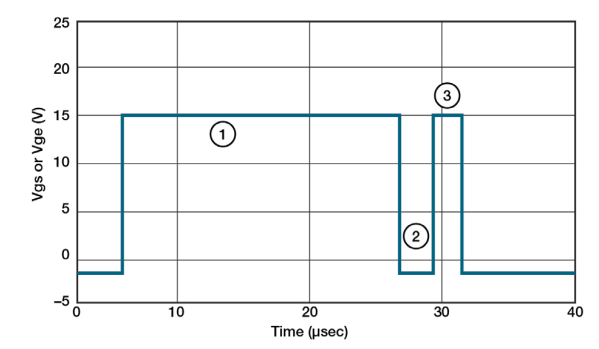
\includegraphics[width=0.8\textwidth]{./Images/Double-Pulse_testing_input.png}
    \caption{Typical Double-Pulse Test Waveform~\cite{DPTest}}
    \label{fig:double_pulse_test_waveform}
\end{figure}

\begin{figure}[h]
    \centering
    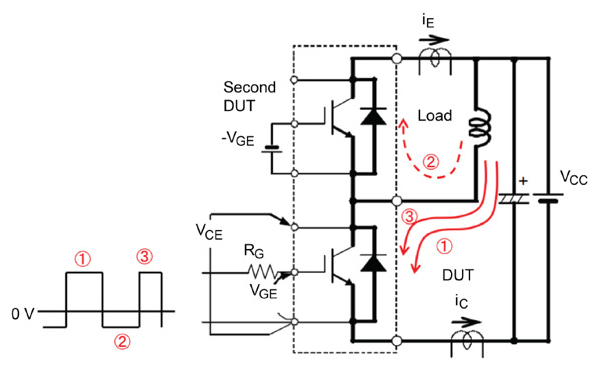
\includegraphics[width=0.8\textwidth]{./Images/Double-Pulse_testing_IGBT.png}
    \caption{Typical Double-Pulse Test Circuit Diagram~\cite{DPTest}}
    \label{fig:double_pulse_test_circuit}
\end{figure}

Unlike the thermal superposition method, double-pulse testing allows for the direct measurement of the switching losses during the transient state of the device, providing more detailed information about the turn-on and turn-off characteristics of the device. This can be particularly useful for devices that are expected to operate under dynamic conditions, such as those found in a buck converter.

The turn-on characteristics of the device can be measured during the second pulse, after the device has been turned off for a short period of time, allowing for the inductor current to freewheel through the diode across the device under test. This means that when the second pulse is applied, the device will still experience a very similar current to the first pulse, allowing for an accurate measurement of the turn-on event.

The method in which the turn-on and turn-off switching losses are extracted from the device during the double-pulse test is by measuring the voltage across the device and the current through the device during the switching events with a high accuracy oscilloscope. By integrating the product of these waveforms over the switching interval, the energy lost during the switching event can be calculated, shown in Equation~\ref{eq:double_pulse_switching_loss}. This equation allows for calculating both the turn-on and turn-off switching losses.
\begin{equation}
    E_{\mathrm{switching}} = \int_{t_1}^{t_2} V(t) \cdot I(t) \, dt
    \label{eq:double_pulse_switching_loss}
\end{equation}

This method also allows for more rapid testing under various operating conditions, as it does not rely on reaching a steady state for accurate measurements. This can be advantageous when testing multiple devices or when testing devices with long thermal constants and can give a bigger picture in how the device performs under different load currents and bus voltages while closely replicating real-world operating conditions.

However, to use this method it requires more complex and expensive equipment such as a high-speed oscilloscope and precise current and voltage probes, which may not be readily available in the testing environment. Additionally, the method doesn't take into consideration the changing characteristics of a switch when operating under different temperatures.
\chapter{Question 2}
\section{2a}
i) This question looks at 2 materials that can be used for the core material of a switched mode transformer, ferrite and nanocrystalline materials. Both of these materials have their own merits and drawbacks when it comes to their use as a core material due to their differing properties which can benefit different applications.

All applications need to be considerate to power losses within the core material, which can be described by the core loss density, \(P_{\mathrm{core}}\), shown in Equation~\ref{eq:core_loss_density}.
\begin{equation}
    P_{\mathrm{core}} = k \cdot f^\alpha \cdot B^\beta
    \label{eq:core_loss_density}
\end{equation}

Some important parameters are needed to be considered when selecting a core material,~\cite{week4Lecture}:
\begin{itemize}
    \item \textbf{Saturation Flux Density} \(B_{\mathrm{sat}}\): This is the maximum magnetic flux density that the core material can handle before it saturates. A higher \(B_{\mathrm{sat}}\) allows for a smaller core size and can improve the efficiency of the transformer.
    \item \textbf{Core Losses}: This includes both hysteresis losses and eddy current losses. Materials with lower core losses are generally preferred for high-frequency applications to improve efficiency.
    \item \textbf{Thermal Stability}: The core material should have good thermal stability to ensure consistent performance under varying temperature conditions, particularly with a high Curie temperature.
    \item \textbf{Relative Permeability} \(\mu_r\): A higher relative permeability allows for better magnetic coupling and can reduce the size of the transformer.
    \item \textbf{Electrical Resistivity}: Higher electrical resistivity can help reduce eddy current losses, which is particularly important at higher frequencies.
\end{itemize}

Ferrites are a type of core material made primarily from dense ceramic iron oxide with other metallic elements. They are widely used for their inexpensive cost, moderate relative permeability, and good performance at high frequencies. Due to their wide adoption within the industry, many different core shapes have also been developed with this material which can leverage some of the properties to enhance wanted behaviours. However, the lower saturation flux density of ferrites can lead to larger core sizes for a given power level in comparison to other materials. Additionally, ferrites can be prone to damage due to their brittle nature. Depending on the application, ferrites can also struggle as when the temperature reaches over 200\(^\circ C\) they can start to lose their magnetic properties, which can lead to a decrease in performance and efficiency of the transformer.

Nanocrystalline materials are another option for transformer core applications. They offer superior performance in terms of lower core losses, due to their higher relative permeability, and higher saturation flux density compared to ferrites. Even with low resistivity within the material it is still able to perform under the right conditions due to its extremely small layers being laminated together which then also combats the eddy current losses within the core and general electrical resistivity. One consequence of the ribbon like construction of the core means that the number of available core geometries for nanocrystalline cores is very limited. However, they tend to be more expensive due to manufacturing complexity. This manufacturing process requires the rapid cooling, million of degrees a second \cite{nanocrystallineManufacture}, and annealing of the material requires specialised equipment and expertise.

Some ranges for the relevant parameters for both materials are shown in Table~\ref{tab:core_materials}, from~\cite{week4Lecture}.

\begin{table}[h]
    \centering
    \caption{Core Material Properties}
    \label{tab:core_materials}
    \begin{tabular}{|c|p{4cm}|p{4cm}|}
        \hline
        \textbf{Parameter} & \textbf{Ferrite} & \textbf{Nanocrystalline} \\
        \hline
        Contents & MnZn, NiZn bulk & 73.5\%-90\% Fe, ribbon thickness-20 \(\mu m\)  \\
        Permeability \(\mu_r\) & \(2000 - 15000\) & \(100000 - 500000\) \\
        Saturation Flux Density, \(B_{\mathrm{sat}}\), T & \(0.3 - 0.45\) & \(1.2 - 1.5\) \\
        Electrical Resistivity, \(\rho\), \(\mu \Omega m\) & \(10^2 - 10^9\) & \(0.4 - 1.2\) \\
        Curie Temperature, \(T_{\mathrm{Curie}}\), \(^\circ C\) & \(125 - 450\) & \(600\) \\
        Core Loss Density, \(P_{\mathrm{core}}\), W/kg & 12 at \(0.2 T/20 kHz \) 60 \(mW/cm^3\) & 5 at \(0.2 T /20kHz\) \\
        Cost & Low & High \\
        \hline
    \end{tabular}
\end{table}

It should be noted that while nanocrystalline cores exhibit lower core losses at 20 kHz, this advantage reduces at higher switching frequencies where the ferrite's higher resistivity can help to reduce eddy current losses.

Due to these characteristics ferrites are preferred for high frequency applications due to the high resistivity limiting eddy current losses, while nanocrystalline materials are competitive at medium frequencies with lower hysteresis losses and higher saturation flux density. 

\vspace{0.5cm}
ii) for this question, similar to the core losses of two materials were looked at, two materials for the chokes of such devices were compared, again ferrite and iron powder core materials.

Within the context of the question, a choke is an inductor used in switched-mode power converters to store and release energy each switching cycle, smoothing the pulsating switch current into a relatively steady DC output current. It carries both a DC bias current from the load and a superimposed AC ripple current from the switching action.

One of the more important parameters to consider when selecting a core material for a choke is the saturation current, \(I_\mathrm{sat}\), and how permeability changes under the application's load DC current. It is important to leave enough overhead in the design to ensure that the choke does not saturate under normal operating conditions along with the AC ripple current when operating the switch to avoid a saturation within the core resulting in a drop in permeability and inductance causing the choke to fail.

Ferrite cores are commonly used in high frequency applications due to their high resistivity which helps reduce eddy current losses. Less of the material is needed to achieve the required inductance due to the high initial permeability in addition to being a low cost material. However, ferrite has a sharp B-H curve, hard saturation, meaning that without an air gap placed into the system can be extremely prone to saturation from small AC ripple currents. Then as a result with the air gap, the overall permeability of the core is reduced which can lead to a larger core size and higher core losses. Additionally, the air gap introduces localised eddy current losses in nearby windings while generating some electromagnetic interference which can cause issues in high-frequency sensitive applications.

Within a ferrite based core with an air gap, the inductance of the choke can be expressed as shown in Equation~\ref{eq:ferrite_choke_inductance}.

\begin{equation}
    \begin{split}
    L &= \frac{N^2 \cdot \mu_0 \cdot A}{l_{\mathrm{air\,gap}} + \frac{l_c}{\mu_r}}\\
    \text{as } l_{\mathrm{air\,gap}} \gg \tfrac{l_c}{\mu_r}, \quad L &\approx \frac{N^2 \cdot \mu_0 \cdot A}{l_{\mathrm{air\,gap}}}
    \end{split}
    \label{eq:ferrite_choke_inductance}
\end{equation}

Iron powder cores are made from finely ground iron particles suspended and bonded within a non conducting material. They have a more gradual B-H curve, soft saturation, compared to ferrites, which means they are less prone to saturation and can handle higher DC bias currents without significant loss of inductance. This makes them suitable for applications where the choke is expected to carry a significant DC current. However, they typically have higher core losses compared to ferrites, especially at high frequencies, due to their lower resistivity which can lead to increased eddy current losses.

Due to the characteristics of the materials, they both suit different applications, with ferrite cores being more suitable for high-frequency applications with lower DC bias currents, while iron powder cores are better suited for applications with higher DC bias currents and lower switching frequencies where the higher core losses are less of a concern

Shown in Table~\ref{tab:choke_core_materials} are some of the relevant parameters for both materials, from~\cite{week4Lecture}.

\begin{table}[h]
    \centering
    \caption{Core Material Properties}
    \label{tab:choke_core_materials}
    \begin{tabular}{|c|p{4cm}|p{4cm}|}
        \hline
        \textbf{Parameter} & \textbf{Ferrite} & \textbf{Iron Powder} \\
        \hline
        Contents & MnZn, NiZn bulk & 90\% Fe bulk  \\
        Permeability \(\mu_r\) & \(2000 - 15000\) & \(1-500\) \\
        Saturation Flux Density, \(B_{\mathrm{sat}}\), T & \(0.3 - 0.45\) & \(1 - 1.3\) \\
        Electrical Resistivity, \(\rho\), \(\mu \Omega m\) & \(10^2 - 10^9\) & varies by grade \\
        Curie Temperature, \(T_{\mathrm{Curie}}\), \(^\circ C\) & \(125 - 450\) & \(700\) \\
        Core Loss Density, \(P_{\mathrm{core}}\), W/kg & 12 at \(0.2 T/20 kHz \) 60 \(mW/cm^3\) & varies by grade \\
        Cost & Low & Low \\
        \hline
    \end{tabular}
\end{table}
\section{2b}

This question looks at the design of half wave rectifier with the following parameters with the circuit shown in Figure~\ref{fig:half_wave_rectifier}.
\begin{itemize}
    \item Input voltage: 230 V AC
    \item Load resistance: 500 \(\Omega\)
    \item Thyristor trigger angle: 65\(^\circ\)
\end{itemize}

\begin{figure}[h]
    \centering
    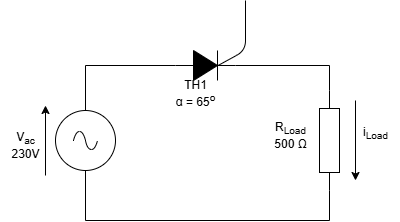
\includegraphics[width=0.4\textwidth]{./Images/rectifierCircuit.png}
    \caption{Question 2b Rectifier Circuit}
    \label{fig:half_wave_rectifier}
\end{figure}

The average voltage for this half wave rectifier can be calculated using the formula shown in Equation~\ref{eq:average_voltage}, \cite{topic8Lecture}.

\begin{equation}
    V_{\mathrm{avg}} = \frac{1}{2\pi} \int_{\alpha}^{\pi} V_{\mathrm{peak}} \sin(\omega t) \, d(\omega t)
    \label{eq:average_voltage}
\end{equation}

Where \(v_{\mathrm{peak}}\) is the peak voltage of the input AC signal, which can be calculated from the RMS voltage as shown in Equation~\ref{eq:peak_voltage}.
\begin{equation}
    v_{\mathrm{peak}} = v_{\mathrm{RMS}} \cdot \sqrt{2} = 230 \cdot \sqrt{2} \approx 325.27\,\mathrm{V}
    \label{eq:peak_voltage}
\end{equation}

Plugging the values into the average voltage equation, the average voltage can be calculated as shown in Equation~\ref{eq:average_voltage_calculation}.
\begin{equation}
    \begin{split}
        v_{\mathrm{avg}} &= \frac{1}{2\pi} \int_{65^\circ}^{180^\circ} 325.27 \sin(\omega t) \, d(\omega t) \\
        &= \frac{325.27}{2\pi} [-\cos(\omega t)]_{65^\circ}^{180^\circ} \\
        &= \frac{325.27}{2\pi} [1 + \cos(65^\circ)] \\
        &\approx 73.66\,\mathrm{V}
    \label{eq:average_voltage_calculation}
    \end{split}
\end{equation}

With the average voltage calculated, the average current through the load can be calculated using Ohm's law as shown in Equation~\ref{eq:average_current}.
\begin{equation}
    i_{\mathrm{avg}} = \frac{v_{\mathrm{avg}}}{R} = \frac{73.66}{500} \approx 0.1473\,\mathrm{A}
    \label{eq:average_current}
\end{equation}
\section{2c}

This question looks at finding the junction temperature of a MOSFET with the parameter shown in Table~\ref{tab:question2c}.
\begin{table}[htbp]
    \centering
    \caption{Parameters for Question 2c}
    \label{tab:question2c}
    \begin{tabular}{|l|c|c|}
        \hline
        \textbf{Parameter} & \textbf{Symbol} & \textbf{Value} \\
        \hline
        Ambient temperature & \(T_{\mathrm{amb}}\) & \(20\,^\circ\mathrm{C}\) \\
        MOSFET's \(R_{\mathrm{DS(on)}}\) when at \(20\,^\circ\mathrm{C}\) & \(R_{\mathrm{DS(on)20}}\) & \(25\,\mathrm{m}\Omega\) \\
        RMS current conducted by MOSFET & \(I_{\mathrm{rms}}\) & \(16\,\mathrm{A}\) \\
        Total thermal resistance between MOSFET junction and ambient & \(R_\theta\) & \(7\,^\circ\mathrm{C/W}\) \\
        Coefficient of rise in \(R_{\mathrm{DS(on)}}\) with temperature & \(k_e\) & \(1.1\,\%/^\circ\mathrm{C}\) \\
        \hline
    \end{tabular}
\end{table}

Three equations are needed to be used to find the junction temperature of the MOSFET, shown in Equations~\ref{eq:power_dissipation}, \ref{eq:temperature_rise} and \ref{eq:resistance_temperature}.
\begin{equation}
    P_{\mathrm{cond}} = I_{\mathrm{rms}}^2 \cdot R_{\mathrm{DS(on)}}
    \label{eq:power_dissipation}
\end{equation}
\begin{equation}
    T_{\mathrm{junc}} = T_{\mathrm{amb}} + P_{\mathrm{cond}} \cdot R_\theta
    \label{eq:temperature_rise}
\end{equation}
\begin{equation}
    R_{\mathrm{DS(on)}} = R_{\mathrm{DS(on)20}} \cdot (1 + k_e \cdot (T_{\mathrm{junc}} - T_{\mathrm{amb}}))
    \label{eq:resistance_temperature}
\end{equation}

These equations provide a relationship between the dissipation of power within the MOSFET and how this effect the junction temperature of the device. This then provides a feedback loop as the resistance of the device increases with temperature, which then increases the power dissipation and therefore the temperature further. To find the final junction temperature. By relating each of these equations together, the junction temperature can be found relatively simply. First, the power dissipation can be expressed as a function of the temperature rise as shown in Equation~\ref{eq:power_dissipation_temperature}.
\begin{equation}
    P_{\mathrm{cond}} = I_{\mathrm{rms}}^2 \cdot R_{\mathrm{DS(on)20}} \cdot (1 + k_e \cdot (T_{\mathrm{junc}} - T_{\mathrm{amb}}))
    \label{eq:power_dissipation_temperature}
\end{equation}

Temperature rise can then be expressed as a function of the power dissipation as shown in Equation~\ref{eq:temperature_rise_power}.
\begin{equation}
    T_{\mathrm{junc}} = T_{\mathrm{amb}} + I_{\mathrm{rms}}^2 \cdot R_{\mathrm{DS(on)20}} \cdot (1 + k_e \cdot (T_{\mathrm{junc}} - T_{\mathrm{amb}})) \cdot R_\theta
    \label{eq:temperature_rise_power}
\end{equation}

Substituting in the relevant values into the equation, the final steady state temperature can be calculated as shown in Equation~\ref{eq:final_temperature_calculation}.
\begin{equation}
    \begin{split}
        T_{\mathrm{junc}} &= 20 + 16^2 \cdot 0.025 \cdot (1 + 0.011 \cdot (T_{\mathrm{junc}} - 20)) \cdot 7 \\
        T_{\mathrm{junc}} &= 20 + 44.8 \cdot (1 + 0.011 \cdot (T_{\mathrm{junc}} - 20)) \\
        T_{\mathrm{junc}} &= 20 + 44.8  + 0.4928 \cdot (T_{\mathrm{junc}} - 20) \\
        T_{\mathrm{junc}} - 0.4928 \cdot T_{\mathrm{junc}} &= 64.8 - 9.856 \\
        T_{\mathrm{junc}} &= \frac{54.944}{0.5072} \\
        T_{\mathrm{junc}} &\approx 108.3\,^\circ\mathrm{C}
    \label{eq:final_temperature_calculation}
    \end{split}
\end{equation}

Shown below in Figure~\ref{fig:feedback_loop} is a block diagram showing the feedback loop between the power dissipation and the junction temperature of the device.

\begin{figure}[h]
    \centering
    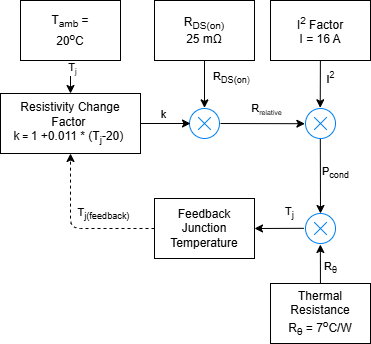
\includegraphics[width=0.6\textwidth]{./Images/Q2c.png}
    \caption{Feedback Loop between Power Dissipation and Junction Temperature}
    \label{fig:feedback_loop}
\end{figure}

\chapter{Question 3}
\section{3a}
This question looks at the calculating various quantities relevant to the design of a dual-switch forward converter. Figure~\ref{fig:forward_converter} shows the circuit diagram for the dual-switch forward converter, from~\cite{EE466CourseworkPart2} and other data is given within Table~\ref{tab:forward_converter_data}. Within this scenario, the converter will be taken as ideal i.e, no forward voltage drop across the diodes.

\begin{figure}[h]
    \centering
    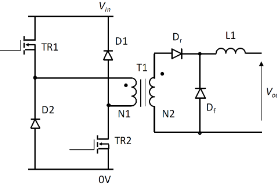
\includegraphics[width=0.6\textwidth]{./Images/forwardConverter.png}
    \caption{Dual-Switch Forward Converter Circuit Diagram~\cite{EE466CourseworkPart2}}
    \label{fig:forward_converter}
\end{figure}

\begin{table}[htbp]
    \centering
    \caption{Parameters for Dual-Switch Forward Converter~\cite{EE466CourseworkPart2}}
    \label{tab:forward_converter_data}
    \begin{tabular}{|c|c|}
        \hline
        \textbf{Parameter} & \textbf{Value} \\
        \hline
        Full-load output power & 50 W \\
        Switching frequency & 120 kHz \\
        L1 inductance & 180 \(\mu\mathrm{H}\) \\
        Transformer T1 turns-numbers \(N_1:N_2\) & 32:28 \\
        Input Voltage & 48 V \\
        Output Voltage & 14 V \\
        \hline
    \end{tabular}
\end{table}

i) Calculate the duty factor at which the converter operates when it is running in the continuous current mode.

To calculate the duty factor for the forward converter, the voltage transfer function for the converter can be used, which is given by Equation~\ref{eq:forward_converter_voltage_transfer},~\cite{MohanConvertersApplicationsDesign}.
\begin{equation}
    \frac{V_{\mathrm{out}}}{V_{\mathrm{in}}} = \frac{N_2}{N_1} \cdot D
    \label{eq:forward_converter_voltage_transfer}
\end{equation}

Plugging in the relevant values into the equation, the duty factor can be calculated as shown in Equation~\ref{eq:duty_factor_calculation}.
\begin{equation}
    D = \frac{V_{\mathrm{out}}}{V_{\mathrm{in}}} \cdot \frac{N_1}{N_2} = \frac{14}{48} \cdot \frac{32}{26} \approx 0.36
    \label{eq:duty_factor_calculation}
\end{equation}
\vspace{0.5cm}

ii) Calculate the minimum voltage that diode \(D_r\) needs to be able to support.

To find the minimum voltage that diode \(D_r\) needs to be able to support, the maximum voltage across the diode during the switching event needs to be calculated. From \cite{Power-Supply-Design-P7}, the maximum voltage across the diode can be expressed as shown in Equation~\ref{eq:diode_voltage} and known values can be used to calculate the output.

\begin{equation}
    \begin{split}
        V_{D_r} &= (V_{\mathrm{in}} 2 \cdot V_f) \frac{N_1}{N_2} -V_f\\
        \text{as } V_f = 0 \quad V_{D_r}  &= V_{\mathrm{in}} \frac{N_1}{N_2} \\
        V_{D_r} &= 48 \cdot \frac{32}{26} \approx 54.86\,\mathrm{V}
        \label{eq:diode_voltage}
    \end{split}
\end{equation}

iii) Calculate the output power at which the converter will enter the boundary conduction mode.

To calculate the output power at which the converter will enter the boundary conduction mode, the ripple current within the inductor needs to be calculated. As this is looking for the boundary conduction mode, the ripple current will be equal to the average current through the inductor, which can be calculated using Equation~\ref{eq:average_inductor_current} and subsequently substituting in the known values.
\begin{equation}
    \begin{split}
        \varDelta i_L &= \frac{(V_\mathrm{in\,sec} - V_\mathrm{out})\cdot D}{f_{sw} \cdot L}\\
        &= \frac{(48 \cdot \frac{26}{32} - 14)\cdot 0.36}{120000 \cdot 180 \cdot 10^{-6}} \approx 0.417\,\mathrm{A}
    \end{split}
    \label{eq:average_inductor_current}
\end{equation}
The final output power at which the converter will enter boundary conduction mode can be calculated using the average inductor current and the output voltage as shown in Equation~\ref{eq:boundary_conduction_power}.
\begin{equation}
    \begin{split}
        P_{\mathrm{boundary}} &= V_{\mathrm{out}} \cdot I_{\mathrm{avg}} = V_{\mathrm{out}} \cdot \frac{\varDelta i_L}{2} \\
            &= 14 \cdot \frac{0.417}{2} \\
            &\approx 2.92\,\mathrm{W}
    \end{split}
    \label{eq:boundary_conduction_power}
\end{equation}

iv) Calculate the flux density swing in the transformer's core material.

To calculate the flux density swing in the transformer's core material. Equation \ref{eq:flux_density_swing} can be used, where \(A_e\) is the effective cross-sectional area of the core, \(V\) is the voltage across the primary winding during the on-time, \(N_1\) is the number of turns in the primary winding and \(f_{sw}\) is the switching frequency.
\begin{equation}
    \begin{split}
        \varDelta B &= \frac{V \cdot D}{N_1 \cdot A_e \cdot f_{sw}} \\
    \end{split}
    \label{eq:flux_density_swing}
\end{equation}

A version of this equation can be found in \cite{FundamentalsOfPowerElectronics} but has been adapted for more simple calculations. For the final flux density swing, the known values are substituted into the equation as shown in Equation~\ref{eq:flux_density_swing_calculation}. The relative cross sectional area of the core was provided from the cores data sheet within \cite{EE466CourseworkPart2}
\begin{equation}
    \begin{split}
        \varDelta B &= \frac{48 \cdot 0.36}{32 \cdot 69\cdot 10^{-6} \cdot 120000} \\
        &\approx 0.065\,\mathrm{T}
    \end{split}
    \label{eq:flux_density_swing_calculation}
\end{equation}

v) Calculate the peak magnetizing current drawn by the transformer.

To calculate the peak magnetizing current drawn by the transformer, the magnetizing inductance needs to be calculated first. The magnetizing inductance can be calculated using the formula shown in Equation~\ref{eq:magnetizing_inductance} \cite{FundamentalsOfPowerElectronics}, where \(L_m\) is the magnetizing inductance, \(N_1\) is the number of turns in the primary winding, \(\mu_0\) is the permeability of free space, \(\mu_r\) is the relative permeability of the core material and \(A_e\) is the effective cross-sectional area of the core.
\begin{equation}
    L_m = \frac{N_1^2 \cdot \mu_0 \cdot \mu_r \cdot A_e}{l_e}
    \label{eq:magnetizing_inductance}
\end{equation}

substituting in the known values into the equation, the magnetizing inductance can be calculated as shown in Equation~\ref{eq:magnetizing_inductance_calculation}. Where needed the core characterstics were taken from the data sheet within \cite{EE466CourseworkPart2}.
\begin{equation}
    \begin{split}
        L_m &= \frac{32^2 \cdot 4\pi \cdot 10^{-7} \cdot 1720 \cdot 69\cdot 10^{-6}}{68\cdot 10^{-3}} \\
        &\approx 2.25\,\mathrm{mH}
    \end{split}
    \label{eq:magnetizing_inductance_calculation}
\end{equation}

This result can then be used to calculate the peak magnetizing current similarly to the flux density swing, by using the voltage across the primary winding during the on-time, the duty factor, the magnetizing inductance and the switching frequency as shown in Equation~\ref{eq:peak_magnetizing_current}.
\begin{equation}
    \begin{split}
        I_{\mathrm{mag\,peak}} &= \frac{V \cdot D}{L_m \cdot f_{sw}} \\
        &= \frac{48 \cdot 0.36}{2.25\cdot 10^{-3} \cdot 120000} \\
        &\approx 0.064\,\mathrm{A}
    \end{split}
    \label{eq:peak_magnetizing_current}
\end{equation}
\section{3b}
This question looks at the control of a high-side MOSFET within a dual-switch forward converter configuration and how it is possible to use a bootstrap and high-voltage level-shifting MOSFET circuit to drive the high-side MOSFET, \cite{BootstrapCircuit}. The reason for this is that the source of the high-side MOSFET does not have a reference point to ground, which makes it difficult to drive the gate of the MOSFET.

A bootstrap circuit is a common method used to drive the high-side MOSFET in a dual-switch forward converter. It commonly consists of a bootstrap capacitor, diode and a resistor. Additions can be made to this circuit such as a high-voltage level-shifting MOSFET. The operation of the bootstrap circuit can be explained in two phases, the charging phase and the discharging phase.

The charging phase occurs when the low-side MOSFET is turned on, pulling the source of the high-side MOSFET to ground. During this time, the bootstrap capacitor is charged through the diode from the supply voltage. The voltage across the bootstrap capacitor will be equal to the supply voltage.

When switching to the discharging phase, the low-side MOSFET is turned off and the high-side MOSFET is turned on. During this time, the source of the high-side MOSFET is pulled up to the supply voltage, which allows the bootstrap capacitor to provide the necessary gate drive voltage to keep the high-side MOSFET on. The voltage across the bootstrap capacitor will decrease as it discharges through the gate of the high-side MOSFET.

Additionally to the bootstrap circuit, a high-voltage level-shifting MOSFET can be used to drive the gate of the high-side MOSFET. This level-shifting MOSFET is used to shift the low-voltage signal from the IC to be able to still control the high-side MOSFET. Depending on the logic required by the gate driver impacts how the level-shifting MOSFET is used, for example, if the gate driver requires a high signal to turn on the high-side MOSFET, the level-shifting MOSFET can be used to pull the input of the gate driver high to have the correct output to drive the high-side MOSFET. The inverse is also true. If the driver needs a low signal to activate the gate then the level-shifting MOSFET can pull it low instead.

Shown below in Figure~\ref{fig:bootstrap_circuit} is an example block diagram showing how the bootstrap circuit and level-shifting MOSFET can be used together to drive the high-side MOSFET in a dual-switch forward converter configuration where the gate driver is modelled after the IR2117 with an active low input.

\begin{figure}[h]
    \centering
    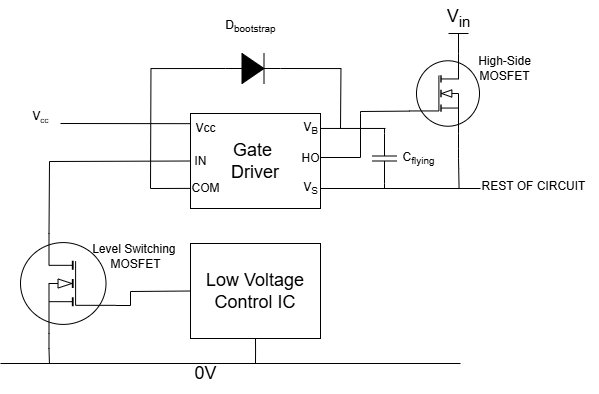
\includegraphics[width = 0.6\textwidth]{./Images/Q3b.png}
    \caption{Block diagram of bootstrap circuit and level-shifting MOSFET}
    \label{fig:bootstrap_circuit}
\end{figure}

\section{3c}
This question looks at redesigning the circuit of the dual-switch forward converter to contain a synchronous rectifier instead of a diode. A synchronous rectifier is a MOSFET that is used in place of a diode to improve the efficiency of the converter by reducing the voltage drop across the rectifying element. This is particularly beneficial in low-voltage, high-current applications where the forward voltage drop of a diode can lead to significant power losses,~\cite{synchronousRectification}.

Shown below in Figure~\ref{fig:synchronous_rectifier} is the redesigned circuit of the dual-switch forward converter with a synchronous rectifier, where the diodes have been replaced by MOSFETs and a gate controller.

\begin{figure}[h]
    \centering
    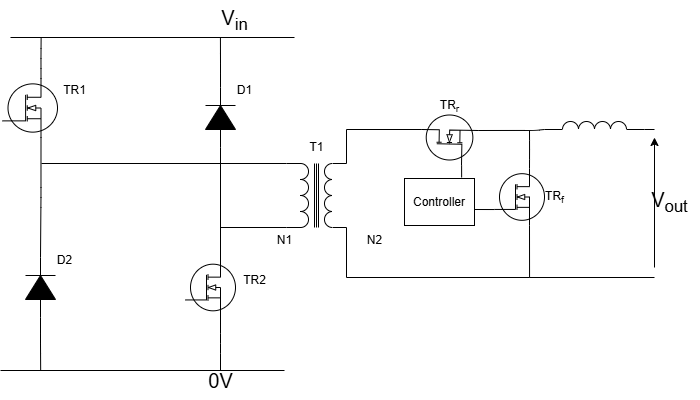
\includegraphics[width=0.6\textwidth]{./Images/Q3c.png}
    \caption{Redesigned Dual-Switch Forward Converter with Synchronous Rectifier}
    \label{fig:synchronous_rectifier}
\end{figure}

This configuration reduces the conduction losses in the rectifying element, as the MOSFET can have a much lower on-resistance compared to the forward voltage drop of a diode. This matters a lot when the output voltage is low and the current is high, as the power loss in the diode can be significant.

The circuit operates similarly to the original dual-switch forward converter, with the main difference being that the synchronous rectifier MOSFETs are controlled by a gate driver that ensures they turn on and off at the appropriate times to mimic the behavior of the diodes they replace. To prevent the sudden onrush of current, shoot through, if both devices end up on at the same time, the gate driver is designed to have dead time between the switching of the two MOSFETs. Conduction can still occur during the dead time due to the body diode of the MOSFETs.

Shown below in Figure~\ref{fig:synchronous_rectifier_waveforms} is a rough sketch of the waveforms for the synchronous rectifier MOSFETs.
\begin{figure}[h]
    \centering
    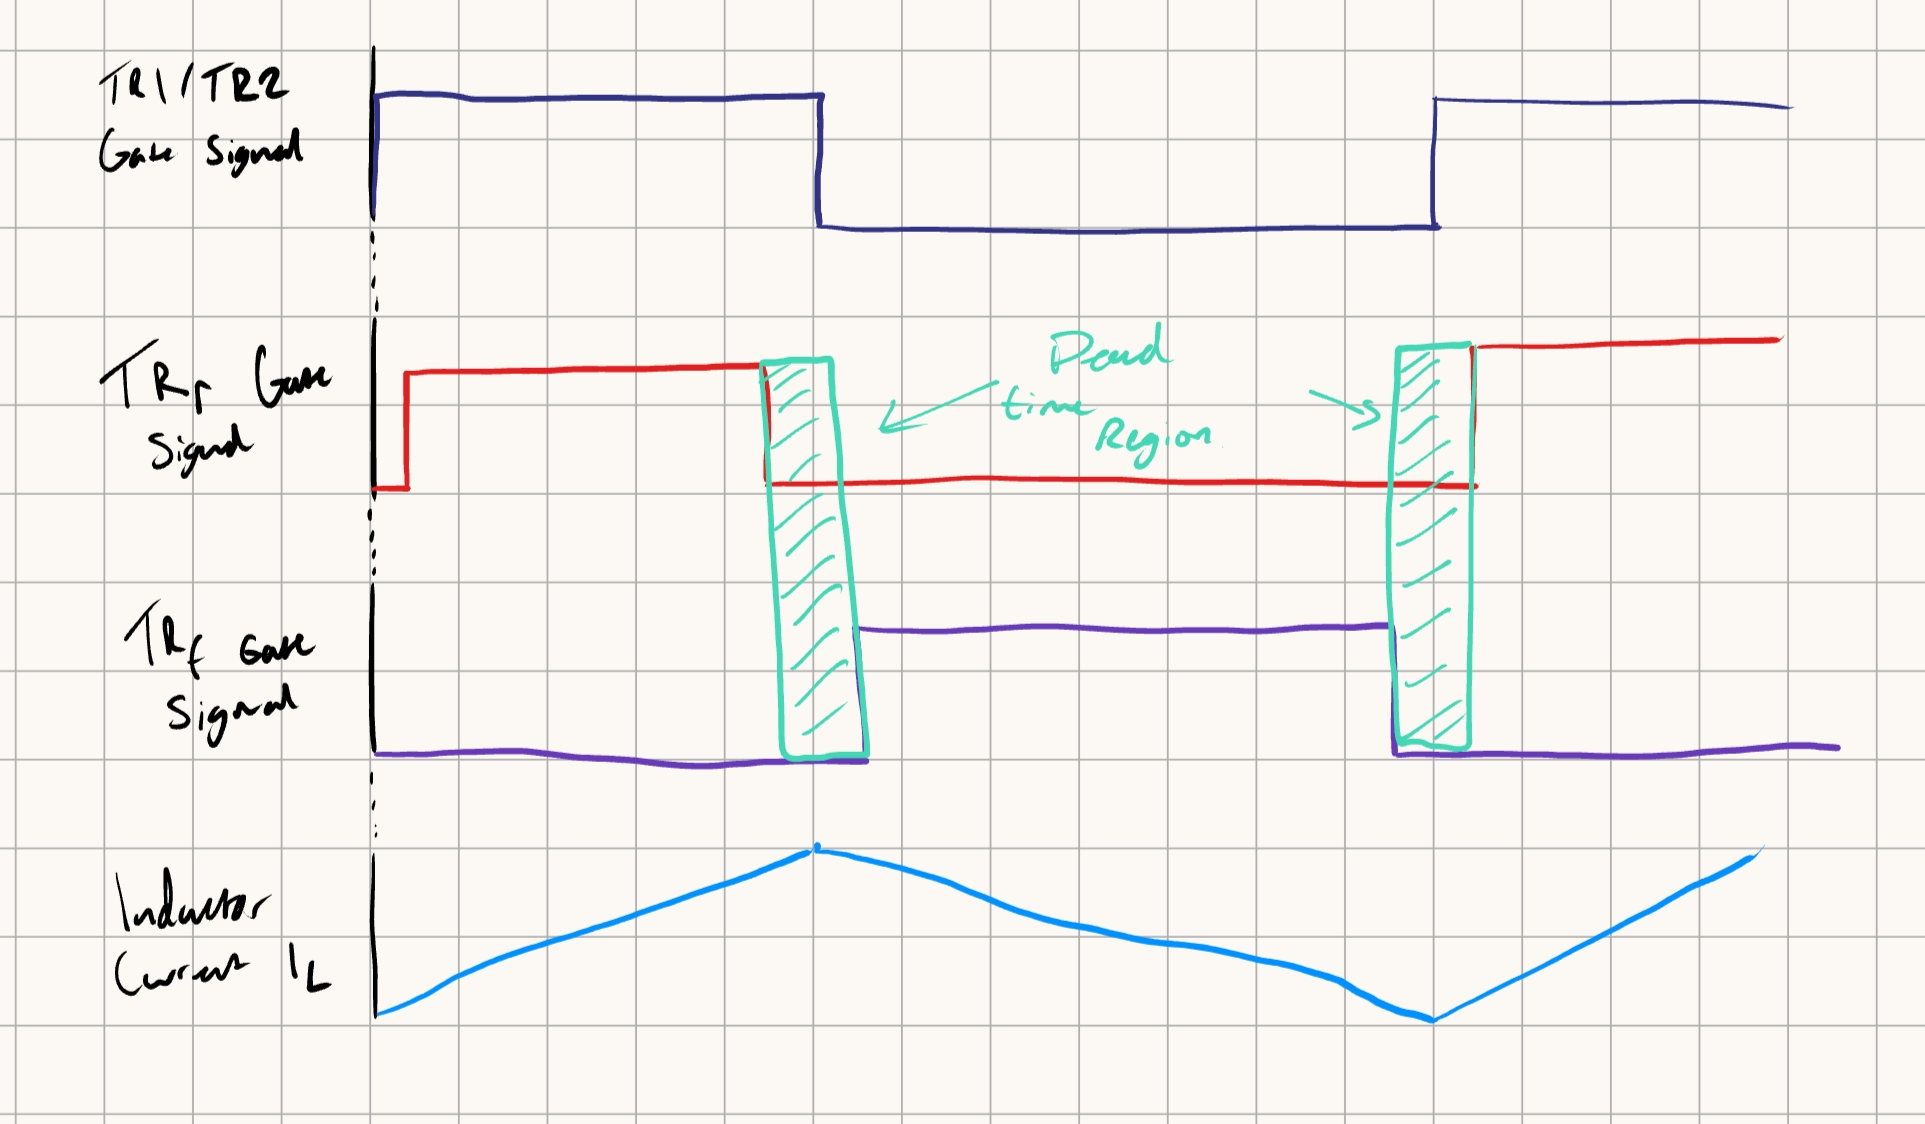
\includegraphics[width=0.6\textwidth]{./Images/Q3c_waveform.jpg}
    \caption{Example waveforms for synchronous rectifier MOSFETs}
    \label{fig:synchronous_rectifier_waveforms}
\end{figure}

\printbibliography
\end{document}